\documentclass[a4paper]{article}

\usepackage{pgfplots}
\usepgfplotslibrary{patchplots}
\pgfplotsset{compat=1.4}

\begin{document}
%too expensive
%\end{document}% disable -- is too expensive
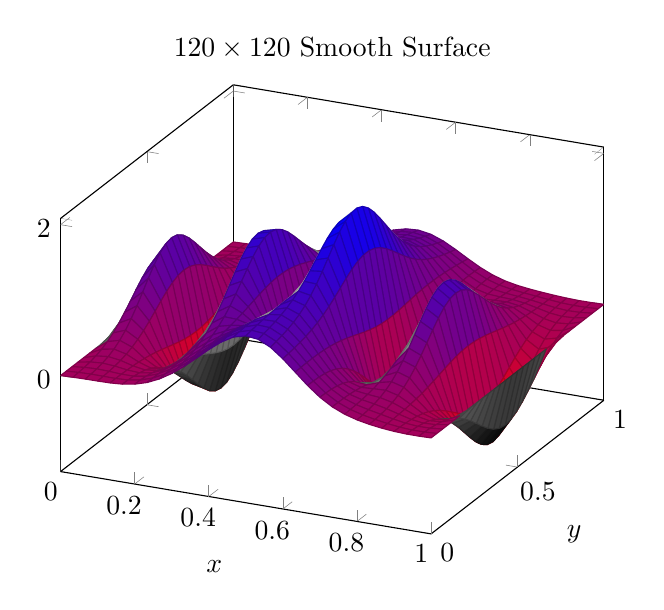
\begin{tikzpicture}
%\tracingmacros=2 \tracingcommands=2
\begin{axis}[
	title=$120 \times 120$ Smooth Surface,
	xlabel=$x$,
	ylabel=$y$]
\addplot3[surf,samples=31,
%	patch to triangles,
	miter limit=1,
%	mesh/show normals=true, mesh/show normals length factor=6, every patch normal/.style={red},
  mesh/interior colormap={blueblack}{color=(red) color=(blue)},
  %mesh/interior colormap thresh=0.1,
  colormap/blackwhite, 
	domain=0:1] 
	{sin(deg(8*pi*x))* exp(-20*(y-0.5)^2) 
	+ exp(-(x-0.5)^2*30 
		- (y-0.25)^2 - (x-0.5)*(y-0.25))};
\end{axis}
\end{tikzpicture}
\end{document}

